\chapter{Architecture}

This chapter describes the architecture of JPaxos.
First the general architecture of the library is presented, consecutively focusing on its parts in detail.
Later the most significant data structures and threading architecture details are presented.

\section{Architecture overview}
\indent\par
Easiest way to understand the architecture of JPaxos is to analyze it's architecture in top-down approach.

\subsection{Processes and their communication}

For JPaxos there are two possible approaches of building replicated services. The first, recommended by us, requires from the service client application using a \texttt{Client} module. The other approach incorporates client module with replica, but it places the responsibility for finding a working replica on the user. The possible approaches are visualised on firure \ref{fig:jpaxos_processes}.

\begin{figure}[h]
 \begin{tabular}{ccc}
  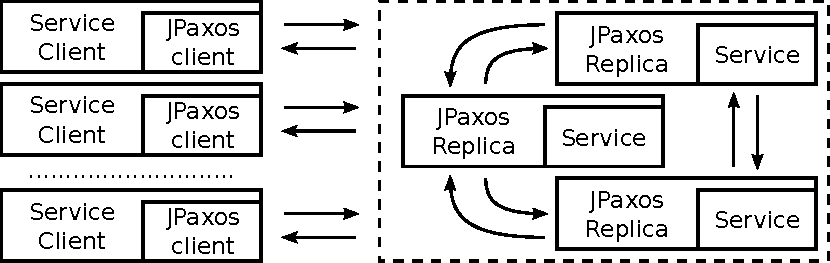
\includegraphics[width=0.44\textwidth]{architecture/userArchitecture1.pdf}
  &
  \hspace{0.02\textwidth}
  &
  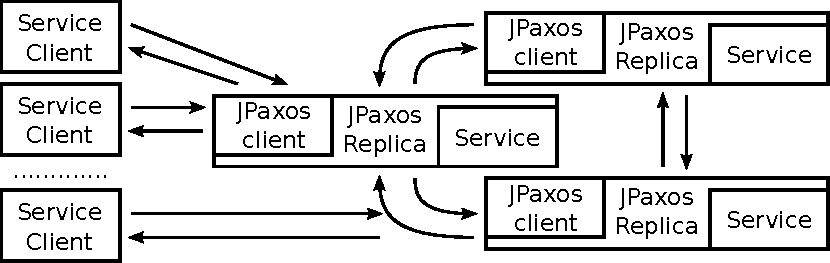
\includegraphics[width=0.44\textwidth]{architecture/userArchitecture2.pdf}
  \\ 
  \scriptsize a) JPaxos client integrated with service client
  & & 
  \scriptsize b) JPaxos client integrated with the replica\\
 \end{tabular}
 \fcmfcaption{Two models of JPaxos}\label{fig:jpaxos_processes}
\end{figure}

The JPaxos \texttt{Client} is responsible for connecting to replicas, providing availability of service as the replica connected with client crashes and ensures that the request will be eventually answered.

Integrating the \texttt{Client} module with service client provides full transparency of replication for the clients.
The service client contacts with the JPaxos \texttt{Client} module as if it would contact with the service -- i.e. it executes requests and gets answers for them.

If one chooses the second approach -- integrating \texttt{Client} in the replica -- the transparency is lost, and the programmer using JPaxos must care for selecting a working replica himself. However, this approach enables using JPaxos in wider context -- for example, one could possibly create a REST web service, and use an usual web client as the service Client, while the service itsel woule be replicated using JPaxos.

The JPaxos Replica module is responsible for global request ordering, passing the requests to the service, answering to the clients and recovering service from crash.

The service itself must be integrates within JPaxos replica. It gets the requests and responds to them. However, in order to make the resource usage bounded JPaxos requires additional functionality from the service, that partialy breaks the transparency - the service must provide snapshots of it's state
once a time, % TODO: lepsze sformuowanie
as well as be able to recover it's state from a snapshot, possibly made by other replica.
As we assume that the services are deterministic, recovering from snapshot originating from other replica is not an issue, however for some services creating a snapshot may present a challenge.

\subsection{Client and client-replica communication}

The JPaxos client module is a single smallweight module that performs several tasks:
\begin{itemize} 
 \item Connects to the replicated service
 \item Reconnects to the replicated service if the connection is lost (e.g. if a replica crashed)
 \item Retreives (or acknowledges) a Client ID for recognising the requests
 \item Sends the requests
 \item Waits for answer, retransmitting the request if needed
\end{itemize}

For the communication with replicas Client uses TCP protocol.

\subsection{Service}

Service is the core part -- in fact it's the service that uses JPaxos for replication.
In order to connect a service with the library, it must implement an interface provided by JPaxos. The interface provides required communication between the library and the service.

The interface for interconnecting JPaxos replica and service allows for:
\begin{itemize}
 \item Executing requests and providing answers for them
 \item Creating Snapshots
 \item Recovering from shansphots
\end{itemize}

\subsection{Replica}

Replica is the most important part of the JPaxos. It consists of numerous modules as depicted on the figure \ref{fig:replica_architecture}.

\begin{figure}[h]
 \centering
 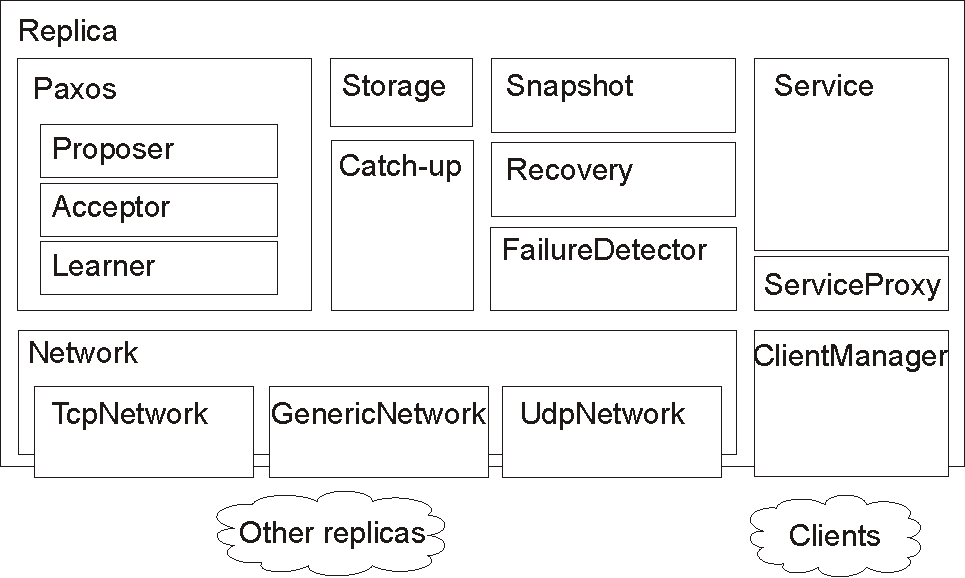
\includegraphics[keepaspectratio, width=0.75\textwidth]{architecture/replica_architecture.pdf}
 \caption{Block diagram of JPaxos modules}
 \label{fig:replica_architecture}
\end{figure}

Short description of the modules of JPaxos goes as follows:

\begin{description}
  \item[Replica ] interconnects other modules - especially the ClientManager, Paxos ans ServiceProxy
  \item[ClientManager ] maintains connection to clients, receives requests from them and forwards the answers
  \item[Paxos ] implements Paxos consensus algorithm
  \begin{description}
    \item[Proposer ] sends new proposes
    \item[Acceptor ] receives proposes and accepts them
    \item[Learner ] collects accepts and decides
  \end{description}
  \item[CatchUp ] takes care for lost ballots as well as retreives the state from othrs by recovery
  \item[SnapshotMaintainer ] controls snapshot mechanism
  \item[Recovery ] chooses proper recovery method and does the actual recovery processes
  \item[Storage ] keeps all the data that do not need to survive crash
  \item[Stable Storage ] keeps the data needed for recovery
  \item[Service Proxy ] as only module contacts with the Service, provides as much transparency as possbible for the service
\end{description}

\begin{TODO}
 Stuff below
\end{TODO}


\section{Storage and data structures}
\label{sec:storage_and_data_structures}

\subsection{Storage and StableStorage interfaces}
\label{subsubsec:storage_and_stablestorage_interfaces}

There are two interfaces containing data for Paxos protocol.

Most of the data is used in multiple classes, but should be accessed only from dispatcher thread (see subsection \ref{sec:threads})

\paragraph{\normalfont \ttfamily lsr.paxos.Storage}
holds all data that are not required for disk-recovery or have been read from a config file.

It also holds some data that could be generated every time used, but as they don't change it's more efficient to have them prepared before.

This class also has the reference on \texttt{StableStorage}.

\begin{description}
\setlength{\itemindent}{0pt}
  \item[]{\tiny\vspace{-0.5em}Config file\vspace{-0.5em}}
    \item[n] Number of processes 
    \item[processes] List of processes
    \item[localID] ID of the replica
  \item[]{\tiny\vspace{-0.5em}Pre-generated\vspace{-0.5em}}
    \item[acceptors] List of processes acting as acceptors
    \item[learners]  List of processes acting as learners
  \item[]{\tiny\vspace{-0.5em}Protocol data\vspace{-0.5em}}
    \item[firstUncommited] First not decided yet instance.
    \item[windowSize] Current size of the window used for multiple instances
    % TODO: ref for multiple instances
\end{description}

\paragraph{\normalfont \ttfamily lsr.paxos.StableStorage} interface is designed to hold all data that must be synchronised with disk.

It is a good practise to keep all data needed for disk recovery in one class, and the StableStorage is such a interface.

The interface currently provides:
\begin{description}
\setlength{\itemindent}{0pt}
  \item[log] the Paxos Log
  \item[snapshot] most recent snapshot
\end{description}


\subsection{The Paxos Log}
\label{subsubsec:the_paxos_log}
The most important data structure, the log, is part of StableStorage.

In our program responsible for that is interface \texttt{lsr.paxos.Log} and class \texttt{lsr.paxos.Con\-sen\-susInstance}.

\texttt{ConsensusInstance} is class keeping all data related to single instance:
\begin{description}
  \setlength{\itemindent}{0pt}
  \item[state] - the instance can be in one of three state:
  \begin{description}
    \setlength{\itemindent}{0pt}
    \item[\tiny UNKNOWN] - no information about current view nor value,
    \item[\tiny KNOWN] - view and value are specified and \textbf{can} be changed later,
    \item[\tiny DECIDED] - view and value are specified and \textbf{cannot} be changed.
  \end{description}
  \item[view] - view of last received message related with this instance,
  \item[value] - the value which is held by this instance (packed requests received from clients which are executed after deciding),
  \item[accepts] - set of known replicas which accepted (view, value) pair.
\end{description}
This class can be easily serialised(deserialised) to(from) byte array to send instances across network. Currently all instance data is saved in RAM memory. When implementing stable storage, this class should be changed.

\texttt{Log} implementations are responsible for managing list of consensus instances. Inside log we have always all instances with id between \textbf{lowestAvailableId}(inclusive) and \textbf{nextId} (exclusive). Instances below \textbf{lowestAvailableId} have already been truncated and instances above \textbf{nextId} are yet unknown. \\New instances can be appended to log and after this operation \textbf{nextId} value is increased by 1. \\Log allows also to retrieve instances from it. There are 3 possible cases when retrieving instance with specified id:
\begin{itemize}
  \item (id $<$ lowestAvailableId) - instance has been truncated and null value is returned,
  \item (lowestAvailableId $\leq$ id $<$ nextId) - instance is inside log so it is returned,
  \item (nextId $\leq$ id) - empty instances between nextId and id are created and empty instance is returned.
\end{itemize}
Old instances can be removed by truncating log and after that lowestAvailableId is increased. 

Appending, retrieving and truncating instances are three main operations performed by log. To perform this operations fast, we have used \texttt{TreeMap} structure for holding all instances.

\subsection{Significant data structures}
\label{subsubsec:significant_structures}
  \begin{description}
    \item[pendingRequests\textless RequestId, Client \textgreater] -- Keeps the requests received from the client for execution that were not yet executed. After execution of request, the reply is sent to client from this structure.
    \item[lastReplies\textless ClientID, Reply\textgreater] -- For each c\-li\-en\-t, keeps the last reply that was sent to it. If client retransmits message which was executed, replica responses immediately.
    \item[decidedWaitingExecution] -- Paxos might d\-e\-cide instance $k$ before instance $k-1$, but the replica must execute all requests in order. So it must cache instance $k$ until all previous instances are decided.
    \item[executedRequests] -- We have to save IDs of all requests which were executed on state machine to prevent executing the same request twice. 
	\item[executedDifference] -- Used to recreate executedRequests structure from moment when snapshot was made by state machine.
  \end{description}


\section{Threads}
\label{sec:threads}

\begin{description}
  \item[Replica] \hfill
    
    Designed as event loop -- waits for new events at certain event queue and reacts on them.

    The event may either be ``instance ordered'', or may concern snapshotting -- new snapshot was made by service, catch-up provided new snapshot or new snapshot is requested from the state machine.

    For most of the time Replica thread waits for requests to be ordered. If they can not be yet executed, puts them on a list (uses for that the decidedWaitingExecution object), when instance executeUB is ordered, replica executes all possible instances.
    
    If there is a client connection waiting for this request, answer is sent to the client.
    
    As for snapshotting -- replica is a proxy ensuring linearizability in snapshot handling.
    Multiple threads (replica itself, dispatcher and catch-up) may therefore safely execute their snapshot-concerning routines.
    
    % Work of the Replica thread could be done by the dispatcher, but executing requests might take some time, which would block the dispatcher thread and therefore the state machine. Like this, there is more parallelism on the framework, as the protocol and the request execution can proceed in parallel.

  \item[Dispatcher] \hfill
    
    Also designed as an event loop, the dispatcher executes Paxos consensus algorithm as well as provides secure access to critical data structures.

    It is responsible for sending, receiving and handling most of the protocol messages. 
    
    Events are placed on the event queue in the following situations:
    
    
    \begin{tabular}{rl}
      FailureDetector & \begin{tabular}[t]{l}
                          suspects another process \\
                          leader sends alive messages
                        \end{tabular} \\
      NetworkListener & \begin{tabular}[t]{l}
                          receives a new message \\
                          sent a message %\footnote{failure detector is informes about each sent message, as it may update timeout for sending alives}
                        \end{tabular} \\
      Paxos.propose() & \begin{tabular}[t]{l}
                          the application starts a new proposal
                        \end{tabular} \\
      Paxos.startProposal() & \begin{tabular}[t]{l}
                                the application asks the current process \\ \hspace{1em} to become a proposer.
                              \end{tabular} \\
      CatchUp &  \begin{tabular}[t]{l}
                   gets and merges log fragment \\
                   received a snapshot form other replica
                 \end{tabular} \\
      SnapshotMaintainer & \begin{tabular}[t]{l}
                             Truncates the log after receiving new snapshot
                           \end{tabular} \\
      
    \end{tabular}


	\item[NioClientManager] \hfill

		Using java.nio package we need only one thread \textsc{SelectorThread} to manage all clients connection. Every time new event occurs (incoming connection waits for accepting, data received from client, data ready to be sent) appropriate action is executed. Current implementation allows easy scaling to more \textsc{SelectorThread}'s to balance the CPU load if one thread wouldn't cope with big number of connections.

	\item[UdpNetwork] \hfill

		One thread responsible for listening on DatagramSocket for datagram packages. Every time new message is received, it is deserialised and all listeners are notified. 

	\item[TcpNetwork] \hfill

		For TCP connection between each two replicas a separate thread is created. Also there is one thread which waits for new incoming connections. Overall we have replica\_count + 1 threads handling TCP. Each of them can be in one of three states:
		\begin{itemize}
			\item connected, waiting for new messages,
			\item not connected, trying to establish new connection,
			\item not connected, waiting for new connection to be established by other replica.
		\end{itemize}

	\item[FailureDetector] \hfill

	 It can work in two states depending whether current replica is leader or not. If leader, failure detector is sending \alive message every amount of time. If the replica is a follower, it waits for new message from leader or for timeout. If any message from leader is received, timer is reset. Otherwise, when timeout occurs, proposer is started.

  \item[CatchUp]\hfill

    This thread manages catch-up process.

    Most of the time it is inactive (sleeping). It activates itself every 2 seconds or when some other thread wakes it up. The thread controls catch-up mechanism (see: \ref{subsec:catch_up_algorithm}) until certain conditions are met (i.e. as long as needed), and suspends itself after then.
    
    Even if the conditions are met at the waking of CatchUp, the thread sends one query for missing instances before deactivating itself.
\end{description}
